\documentclass[10pt]{article}
\usepackage{fullpage}
\usepackage[fleqn]{amsmath}
\usepackage{mathtools}
\usepackage{graphicx}
\usepackage{amsfonts}
\usepackage{float}
\usepackage{listings}
\usepackage{xcolor}
\usepackage{scrextend}
\usepackage{setspace}
\usepackage{braket}
\usepackage{subcaption}
\usepackage{mwe}
\usepackage{titling}
\usepackage {tikz}
\usetikzlibrary {positioning}
\definecolor {processblue}{cmyk}{0.96,.65,0,0}
\usepackage{caption}
\usepackage{makecell}
\singlespacing

\setlength{\droptitle}{-4em}

\DeclarePairedDelimiterX{\infdivx}[2]{(}{)}{%
  #1\;\delimsize\|\;#2%
}

\def\checkmark{\tikz\fill[scale=0.4](0,.35) -- (.25,0) -- (1,.7) -- (.25,.15) -- cycle;}
\newcommand{\infdiv}{D\infdivx}
\DeclarePairedDelimiter{\norm}{\lVert}{\rVert}

\begin{document}

\title{MAP5345: Partial Differential Equations I \\ \vskip .3cm
Homework 2}
\author{David Miller}

\maketitle

\subsection*{Problem 1}
We have the following Taylor Series expansions
$$e^x =  \sum\limits_{n=0}^\infty \frac{x^n}{n!}, \quad cos(x) = (-1)^n\frac{x^{2n}}{(2n)!}, \quad sin(x) = \sum\limits_{n=0}^\infty (-1)^n \frac{x^{2n+1}}{(2n+1)!}$$
Letting $x = i\theta$ we get 
\begin{align*}
e^{i\theta} & = \sum\limits_{n=0}^\infty \frac{(i\theta)^n}{n!} \\
            & = \sum\limits_{m=4n}^\infty \frac{\theta^m}{m!} - \sum\limits_{m=4n+2}^\infty \frac{\theta^m}{m!} + i\bigg(\sum\limits_{m=4n+1}^\infty \frac{\theta^m}{m!} - \sum\limits_{m=4n+3}^\infty \frac{\theta^m}{m!}\bigg) \\
            & = \sum\limits_{m=2n}^\infty (-1)^{m/2}\frac{\theta^m}{m!} + i\bigg(\sum\limits_{m=2n+1}^\infty (-1)^{(m-1)/2}\frac{\theta^m}{m!}\bigg) \\
            & = \sum\limits_{n=0}^{\infty} (-1)^n\frac{\theta^{2n}}{(2n)!} + i\bigg(\sum\limits_{n=0}^\infty (-1)^n\frac{\theta^{2n+1}}{(2n+1)!}\bigg) \\
            & = cos(\theta) + isin(\theta)
\end{align*}
\hfill $\square$

\newpage

\subsection*{Problem 2}
Letting $D$ be the unit cube $[0,1]^3$ and $F  = (x,y,z)$ we get
\begin{align*}
\displaystyle\int_D \nabla \cdot \vec{F} dV & = \int\limits_0^1\int\limits_0^1\int\limits_0^1 \big(\partial_x(x) + \partial_y(y) + \partial_z(z)\big)\,\,dxdydz \\
	& = \int\limits_0^1\int\limits_0^1\int\limits_0^1 3 \,\, dxdydz \\
    & = 3
\end{align*}
\begin{align*}
\displaystyle\int_{\partial D}\vec{F} \cdot \hat{n} \,\, dS & = \int_0^1\int_0^1 (0,y,z) \cdot (-1,0,0) \,\, dydz + \int_0^1\int_0^1 (1,y,z) \cdot (1,0,0) \,\, dydz \\ 
	& + \int_0^1\int_0^1 (x,y,z) \cdot (0,-1,0) \,\,dxdz + \int_0^1\int_0^1 (x,y,z) \cdot (0,1,0) \,\, dxdz \\
    & + \int_0^1\int_0^1 (x,y,z) \cdot (0,0,-1) \,\, dxdy + \int_0^1\int_0^1 (x,y,z) \cdot (0,0,1) \,\, dxdy \\
    & = 3 \bigg(\int_0^1\int_0^1 0 \,\, dS + \int_0^1\int_0^1 1 \,\, dS\bigg) \\
    & = 3
\end{align*}
Now letting $D$ be the unit cube $S^2$ and using the coordinate transformation 
$$x = rsin(\theta)cos(\phi), \quad y = rsin(\theta)sin(\phi), \quad z = rcos(\theta)$$
we get the following
\begin{align*}
\displaystyle\int_D \nabla \cdot \vec{F} dV & = \int_{D} \big(\partial_x(x) + \partial_y(y) + \partial_z(z)\big) \,\, dV \\
	& = 3 \int_D dV \\
    & = 4\pi
\end{align*}
\begin{align*}
\int_{\partial D} \vec{F} \cdot \hat{n} \,\, dS & = \int_{\partial D} \big((x,y,z) \cdot (sin(\theta)cos(\phi), sin(\theta)sin(\phi), cos(\theta))\big) \\
& = \int_{\partial D}\big((sin(\theta)cos(\phi), sin(\theta)sin(\phi), cos(\theta)) \cdot (sin(\theta)cos(\phi), sin(\theta)sin(\phi), cos(\theta)) \big) \,\, dS \\
& = \int_{\partial D} | r | \,\, dS \\ 
& = 4\pi
\end{align*}
where we have used the fact that the volume of a sphere is $\frac{4}{3}\pi r^3$ and the area is $4\pi r^2$.\hfill $\square$

\newpage

\subsection*{Problem 3}
(a) We have the IBVP PDE
\begin{flalign*}
&\partial_tu = k\partial_{xx}u, \quad x \in (0,L), t \geq 0 \\
&u(x,0) = u_0(x) = 2sin(\pi x/L) - 0.5sin(2\pi x/L) + 0.2sin(3\pi x/L) \\
&u(0,t) = u(L,t) = 0
\end{flalign*}
Assuming it has a solution of the form $u(x,t) = X(x)T(t)$ and plugging this into the PDE we get
\begin{align*}
& X(x)T^\prime(t) = kX^{\prime\prime}(x)T(t)
\end{align*}
The only way that the above is possible is when both the RHS and LHS equal some constant $-\lambda$. Using this fact and simplifying we are left with
\begin{align*}
\frac{1}{kT(t)}\frac{\partial T}{\partial t} = \frac{1}{X(x)}\frac{\partial^2X}{\partial x^2} = -\lambda
\end{align*}
These differential equation $T(t)$ has the solution
\begin{align*}
& T(t) = ce^{-\lambda kt}
\end{align*}
while $X(x)$ can take on 3 different solutions
\begin{align*}
& \underline{\text{Case } 1: \lambda > 0} \\
& X(x) = c_1cos(\sqrt{\lambda}x) + c_2sin(\sqrt{\lambda}x) \\
& X(0) = 0 \Rightarrow c_1 = 0 \\
& X(L) = 0 \Rightarrow \lambda_n = \frac{n^2\pi^2}{L^2}, \quad n = 1, 2, 3 \ldots \\
& \Rightarrow X(x) = c_2sin(n\pi x/ L) \\ 
& \underline{\text{Case } 2: \lambda = 0} \\
& X(x) = c_1x + c_2 \\
& X(0) = 0 \Rightarrow c_2 = 0 \\
& X(L) = 0 \Rightarrow c_1 = 0 \\
& \Rightarrow X(x) = 0 \\
& \underline{\text{Case } 3: \lambda < 0} \\
& X(x) = c_1cosh(\sqrt{-\lambda}x) + c_2sinh(\sqrt{-\lambda}x) \\
& X(0) = 0 \Rightarrow c_1 = 0 \\
& X(L) = 0 \Rightarrow c_2 = 0 \\
& \Rightarrow X(x) = 0
\end{align*}
Case 1 is the only one that does not return the trivial solution. Therefore our product solution is
\begin{align*}
u_n(x,t) = B_nsin(\frac{n\pi x}{L})e^{-\frac{n^2\pi^2}{L^2} kt}
\end{align*}
By the Principle of Superposition we obtain the general solution
\begin{align}
u(x,t) = \sum\limits_{n=1}^\infty B_nsin(\frac{n\pi x}{L})e^{-\frac{n^2\pi^2}{L^2} kt}
\end{align}
To satisfy $u_0(x)$ we have that $B_1 = 2$, $B_2 = -0.5$, $B_3 = 0.2$, and $B_n = 0$ otherwise. Putting all this together, we get that the solution to our IBVP is 
\begin{align}
u(x,t) = 2sin(\frac{\pi x}{L})e^{-\frac{\pi^2}{L^2} kt} - 0.5sin(\frac{2\pi x}{L})e^{-\frac{4\pi^2}{L^2} kt} + 0.2sin(\frac{3\pi x}{L})e^{-\frac{9\pi^2}{L^2} kt}
\end{align}

\begin{figure}[h]
\centering
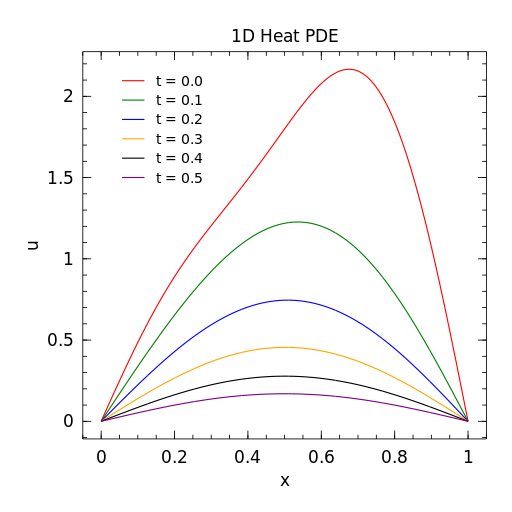
\includegraphics[width=10cm]{HW2_3a.png}
\caption{Numerical representation of solution (1)}
\end{figure}

\noindent Figure 1 shows plots the solution (1) at different time values. As we can see $u(x,t) \rightarrow 0$ as $t \rightarrow \infty$ as we expected. This is because heats dissipates on any object and reaches the equilibrium temperature zero. We can also see that $u(x,t)$ tends to a damped sin graph which is due to heat distribution becoming uniform over our domainx.

\newpage

\noindent (b) Now we are given parabolic initial condition 
\begin{align*}
u_0(x) = x(L-x)
\end{align*}
which we can use to find our coefficient $B_n$. As we do later in problem 4, we take the inner product of both sides with respect to the eigenfunction $X_n = sin(\frac{n\pi x}{L})$. Doing so yields 
\begin{align*}
B_n & = \frac{2}{L}<u_0(x), X_n> \\
& = \frac{2}{L}\int\limits_0^L x(L-x)sin(\frac{n\pi x}{L}) dx \\
& = \frac{2}{L}\int\limits_0^L xLsin(\frac{n\pi x}{L}) dx - \frac{2}{L}\int\limits_0^L x^2sin(\frac{n\pi x}{L}) dx \\
& = 2\bigg(-\frac{xL}{n\pi}cos(\frac{n\pi x}{L})\bigg\vert_0^L + \frac{L}{n\pi}\int\limits_0^L cos(\frac{n\pi x}{L}) dx \bigg) - \frac{2}{L}\bigg(-x^2\frac{L}{n\pi}cos(\frac{n\pi x}{L})\bigg\vert_0^L - 
\frac{2L}{n\pi}\int\limits_0^L xcos(\frac{n\pi x}{L}) dx\bigg) \\ 
& = 2\bigg(\frac{2L^2}{n\pi} + \frac{L^2}{n\pi}sin(\frac{n\pi x}{L})\bigg\vert_0^L\bigg) - \frac{2}{L}\bigg(\frac{2L^3}{n\pi} - \frac{2L}{n\pi}\bigg(\frac{xL}{n\pi}sin(\frac{n\pi x}{L})\bigg\vert_0^L - \frac{L}{n\pi}\int\limits_0^L sin(\frac{n\pi x}{L}) dx\bigg)\bigg) \\
& = \frac{4L^2}{n\pi} - \frac{2}{L}\bigg(\frac{2L^3}{n\pi} - \frac{2L}{n\pi}\bigg(-\frac{L^2}{n^2\pi^2}cos(\frac{n\pi x}{L})\bigg\vert_0^L\bigg)\bigg) \\ 
& = \frac{4L^2}{n\pi} - \frac{2}{L}\bigg(\frac{2L^3}{n\pi} - \frac{2L}{n\pi}\bigg(\frac{2L^2}{n^2\pi^2}\bigg)\bigg) \\
& = \frac{4L^2}{n\pi} - \frac{2}{L}\bigg(\frac{2L^3}{n\pi} - \frac{4L^3}{n^3\pi^3}\bigg) \\
& = \frac{8L^2}{n^3\pi^3} \\
\end{align*}

\newpage

\begin{figure}[h]
\centering
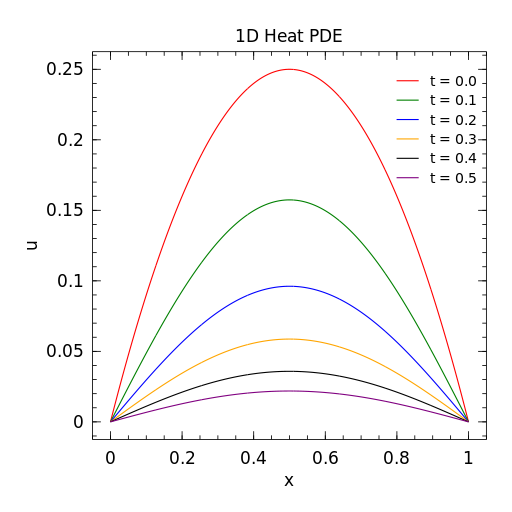
\includegraphics[width=8cm]{HW2_3b.png}
\caption{Numerical representation of 1D Heat Equation with parabolic initial condition}
\end{figure}

\noindent The above graph had a truncation at $N = 1000$ However, truncation values $N \geq 3$ have little visual difference from figure 2.

\begin{figure}[h]
\centering
\begin{minipage}{.5\textwidth}
  \centering
  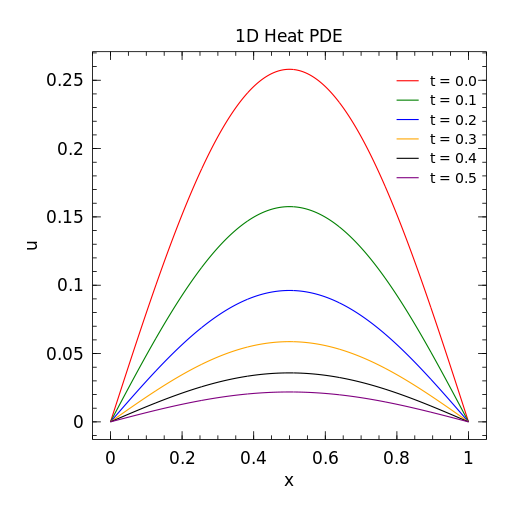
\includegraphics[width=.8\linewidth]{HW2_3b1.png}
  \caption*{Truncation N = 1}
  \label{fig:test1}
\end{minipage}%
\begin{minipage}{.5\textwidth}
  \centering
  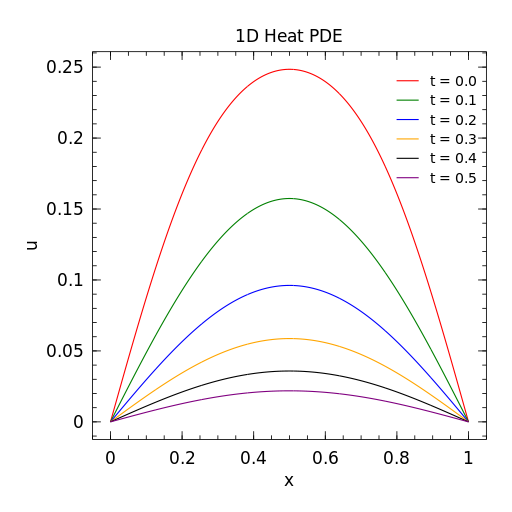
\includegraphics[width=.8\linewidth]{HW2_3b2.png}
  \caption*{Truncation N = 2}
  \label{fig:test2}
\end{minipage}
\end{figure}

\noindent We see that we can essentially truncate at N = 3 because $\vert B_ne^(\frac{-kn^2\pi^2}{L^2}) \vert$ $\approx$ $10^{-20}$ for $n = 3$ (only odd $n$ contribute). This means that there are very small contributions to $u(x,t)$ for any $N \geq 2$. 

\newpage

\subsection*{Problem 4}
(a) Assume that $u(x,t)$ and $v(x,t)$ solve the wave equation. Now let $w(x,t) = \alpha u(x,t) + \beta v(x,t)$ and take partial derivatives
\begin{align*}
& w_t = \alpha u_t + \beta v_t, \quad && w_{tt} = \alpha u_{tt} + \beta v_{tt} \\
& w_x = \alpha u_x + \beta v_x, \quad && w_{xx} = \alpha u_{xx} + \beta v_{xx}
\end{align*}
Plugging into the wave equation we get
\begin{align*}
& w_{tt} - c^2w_{xx} = 0 \Rightarrow \\
& (\alpha u_{tt} + \beta v_{tt}) - c^2(\alpha u_{xx} + \beta v_{xx}) \Rightarrow \\
& (\alpha u_{tt}  + c^2\alpha u_{xx}) + (\beta v_{tt} -c^2\beta v_{xx}) \Rightarrow \\
& \alpha(u_{tt}  + c^2 u_{xx}) + \beta(v_{tt} -c^2 v_{xx}) = \alpha(0) + \beta(0) = 0 
\end{align*}
\hfill $\square$ \\
(b) The wave equation is given by
\begin{align*}
& \partial_{tt}u = c^2\partial_{xx}u, \quad x \in (0,L), t \geq 0 \\
& u(0,t) = u(L,t) = 0 \\
& u(x,0) = u_0(x) \\
& u_t(x,0) = \dot{u}_0(x)
\end{align*}
Now we assume that the solution has the form $u(x,t) = X(x)T(t)$ and plug back into the PDE and get
\begin{align*}
\frac{1}{X(x)}\frac{\partial^2X}{\partial x^2} = \frac{1}{c^2T(t)}\frac{\partial^2T}{\partial t^2} = \lambda
\end{align*}
for some constant $\lambda$. The solution for $X(x)$ is the same eigenvalue problem solved in problem 3. Therefore we have the same countable set of solutions
\begin{align*}
X_n(x) = csin(\frac{n \pi x}{L}), \quad \lambda_n = \frac{n^2\pi^2}{L^2}, \quad n = 1,2,3\ldots
\end{align*}
The time function $T(t)$ is solved similarly in problem 3 where we consider the cases $\lambda > 0$, $\lambda = 0$, and $\lambda < 0$. The only difference is that we do not have explicit initial conditions so we are left with 
\begin{align*}
T_n(t) = c_1cos(\frac{cn\pi t}{L}) + c_2sin(\frac{cn\pi t}{L}), \quad \lambda_n = \frac{c^2n^2\pi^2}{L^2}, \quad n = 1,2,3\ldots
\end{align*}
Putting all this together we get 
\begin{align*}
u(x,t) = \sum\limits_{n=1}^\infty \bigg(A_ncos(\frac{cn\pi t}{L}) + B_nsin(\frac{cn\pi t}{L})\bigg)sin(\frac{n\pi x}{L})
\end{align*}
Using the two initial conditions we get 
\begin{align*}
& u_0(x) = \sum\limits_{n=1}^\infty A_nsin(\frac{n\pi x}{L}) \\
& \dot{u}_0(x) = \sum\limits_{n=1}^\infty \frac{cn\pi}{L}B_nsin(\frac{n\pi x}{L})
\end{align*}
To determine $A_n$ and $B_n$ we take inner products with respect to the eigenfunction $X_m = sin(m\pi x/L)$. 
\begin{align*}
\int\limits_{0}^L u_0(x) X_m dx & = \int\limits_0^L \sum\limits_{n=1}^\infty A_nX_nX_m \\
& = \sum\limits_{n=1}^\infty A_n \int\limits_0^L X_n X_m dx
\end{align*}
\begin{align*}
\int\limits_{0}^L \dot{u}_0(x) X_m dx & = \int\limits_0^L \sum\limits_{n=1}^\infty \frac{cn\pi}{L}B_nX_nX_m \\
& = \sum\limits_{n=1}^\infty \frac{cn\pi}{L}B_n \int\limits_0^L X_n X_m dx
\end{align*}
To simplify the expressions we determine the inner product $<X_n,X_m>$ over the $L^2$ norm
\begin{align*}
<X_n,X_m> & = \int\limits_0^L X_nX_m dx \\
& = \int\limits_0^L \frac{e^{in\pi x/ L} - e^{-in\pi x/ L}}{2i}\frac{e^{im\pi x/ L} - e^{-im\pi x/ L}}{2i} dx \\ 
& = -\frac{1}{4}\int\limits_0^L e^{i(n+m)\pi x / L} + e^{-i(n+m)\pi x / L} - e^{i(m-n)\pi x / L} - e^{i(n-m)\pi x / L} dx \\
& = -\frac{L}{2(n+m)\pi}\int\limits_0^L \frac{e^{i(n+m)\pi x / L} + e^{-i(n+m)\pi x / L}}{2}dx + \frac{L}{2(m-n)\pi}\int\limits_0^L \frac{e^{i(m-n)\pi x / L} + e^{i(n-m)\pi x / L}}{2}dx \\ 
& = \frac{L}{2\pi}\bigg(\frac{sin(\frac{(m-n)\pi x}{L})}{m-n} - \frac{sin(\frac{(m+n)\pi x}{L})}{m+n}\bigg) = 0, \quad m \neq n \\
<X_n, X_n> & = \int\limits_0^L X_n^2 dx \\ 
& = \int\limits_0^L \frac{e^{in\pi x/ L} - e^{-in\pi x/ L}}{2i}\frac{e^{in\pi x/ L} - e^{-in\pi x/ L}}{2i} dx \\ 
& = -\frac{1}{4}\int\limits_0^L -2 + e^{2in\pi x / L} + e^{-2in\pi x / L} dx \\ 
& = \frac{x}{2}\bigg\vert_0^L -\frac{L}{2n\pi}\int\limits_0^L \frac{e^{2in\pi x / L} + e^{-2in\pi x / L}}{2} dx \\ 
& = \frac{L}{2} -\frac{L}{2n\pi}sin(\frac{n\pi x}{L})\bigg\vert_0^L = \frac{L}{2}, \quad m = n
\end{align*}
From this we can conclude that 
\begin{align*}
& A_n = \frac{<u_0(x), X_n>}{<X_n, X_n>} = \frac{2}{L}<u_0(x),X_n> 
& B_n = \frac{L}{cn\pi}\frac{<\dot{u}_0(x), X_n>}{<X_n, X_n>} = \frac{2}{cn\pi}<\dot{u}_0(x), X_n>
\end{align*}
Giving us the desired general solution
\begin{align}
& u(x,t) = \sum\limits_{n=1}^\infty \bigg(A_ncos(\frac{cn\pi t}{L}) + B_nsin(\frac{cn\pi t}{L})\bigg)sin(\frac{n\pi x}{L}), \\
& A_n = \frac{2}{L}<u_0(x),X_n>, \quad B_n = \frac{2}{cn\pi}<\dot{u}_0(x), X_n>
\end{align}
\newline
(c) We are given initial conditions 
\begin{align*}
& u(x,0) = x(L-x) \\
& u_t(x,0) = 0
\end{align*}
and from this we can find the solution to (3) by determining $A_n$ and $B_n$ by plugging our initial conditions into (4). Doing so gets us
\begin{align*}
A_n & = \frac{2}{L} <u_0(x), X_n> \\
& = \int\limits_0^L x(L-x)sin(\frac{n\pi x}{L}) dx \\
& = \frac{8L^2}{n^3\pi^3}, \quad \text{(see problem 3)} \\
B_n & = \frac{2}{cn\pi}<\dot{u}_0(x), X_n> \\
& = \int\limits_0^L 0 dx = 0
\end{align*}
Plugging back into the general solution (3) we get the desired result
\begin{align*}
u(x,t) = \sum\limits_{n=0}^\infty A_ncos(\frac{cn\pi t}{L})sin(\frac{n \pi x}{L}), \quad A_n = \frac{8L^2}{n^3\pi^3}
\end{align*}
(d) To plot the solution to the wave equation for $L = 5$ and $c = 100$, I used the code Dr. Moore has on his personal website. I did this because my personal code was not plotting the solution correctly, but the main idea behind both coding solutions are the same.

\newpage

\begin{figure}[h]
\centering
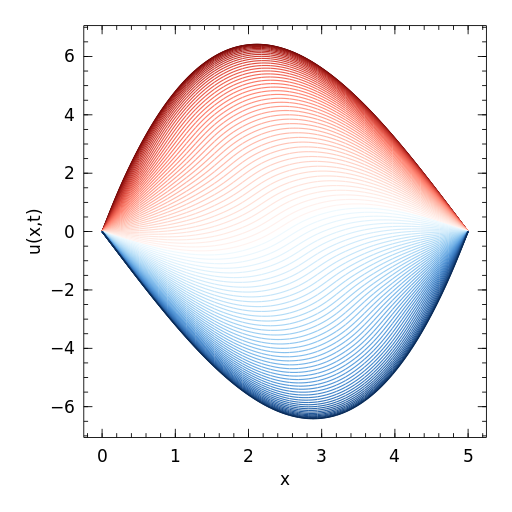
\includegraphics[width=10cm]{wave.png}
\caption{Numerical representation of 1D Wave Equation}
\end{figure}

\end{document}
